
\documentclass[acmtog]{acmart}
% Title portion
\usepackage{indentfirst}
\setlength{\parindent}{2em}
\usepackage{listings}

\title{Assignment 1 : Creating your own OpenGL program} 
\author{Name:\quad WenJi Liu  \\ student number:\quad 13611756
	\\email:\quad liuwj@shanghaitech.edu.cn}

% Document starts
\begin{document}
\maketitle

\vspace*{2 ex}


\section{Introduction}
 In this technical report, i draw basic shapes such as tetrahedron, cubes and spheres, and then shade them with Phong lighting. \\ Besides, i implement the methods supporting object manipulating (such as rotation and translation)and camera controling (also rotation and translation). 
 \par Finally, i enabled the multi-sample antialiasing, face culling and Z-test to give a realistic picture. 
\par Besides, on the rendering part, i use a shader program to implement phong light model. Object manipulating is implemented by changing the model matrix. Camera controlling is implemented by setting PMV matrix over the shaders of objects .
\section{Implementation Details}
\subsection{Intialization}
To draw a object, instead of using glBegin() and glEnd(), i use the VAO,VBO and EBO to lower the cost of rendering.\par First take the tetrahedron as example.
\begin{lstlisting}[frame=single,breaklines=true,language=c++,basicstyle=\footnotesize\ttfamily]
unsigned int terta_VAO, terta_VBO, terta_EBO;
glGenVertexArrays(1, &terta_VAO);
glGenBuffers(1, &terta_VBO);
glGenBuffers(1, &terta_EBO);
\end{lstlisting}
\par Setting up vertices and indices.
\begin{lstlisting}[frame=single,breaklines=true,language=c++,basicstyle=\footnotesize\ttfamily]
GLfloat terta_vertices[] = {
	2,0,0,
	3,0,0,
	2.5,1,-0.5,
	2.5,0,-1,
};
unsigned int terta_indices[] = {0,1,2,1,3,2,0,3,1,0,2,3};
\end{lstlisting}
\par Then  i set up VAO,VBO and bind element array buffer.
\begin{lstlisting}[frame=single,breaklines=true,language=c++,basicstyle=\footnotesize\ttfamily]
glBindVertexArray(terta_VAO);
glBindBuffer(GL_ARRAY_BUFFER, terta_VBO);
glBufferData(GL_ARRAY_BUFFER, sizeof(terta_vertices), terta_vertices, GL_STATIC_DRAW);
glBindBuffer(GL_ELEMENT_ARRAY_BUFFER, terta_EBO);
glBufferData(GL_ELEMENT_ARRAY_BUFFER, sizeof(terta_indices), terta_indices, GL_STATIC_DRAW);
glVertexAttribPointer(0, 3, GL_FLOAT, GL_FALSE, 3 * sizeof(float), (void*)0);
glEnableVertexAttribArray(0);
glBindBuffer(GL_ARRAY_BUFFER, 0);
glBindVertexArray(0);
\end{lstlisting}
\par The main difference in drawing cubes and spheres is that i want to have light shading on them while i just use tetrahedron to be the light source.\par Thus setting up the normals of vertices is required.To acheive that, i have to redefine how the shader explains data input.
\begin{lstlisting}[frame=single,breaklines=true,language=c++,basicstyle=\footnotesize\ttfamily]
glVertexAttribPointer(0, 3, GL_FLOAT, GL_FALSE, 6 * sizeof(float), (void*)0);
glVertexAttribPointer(1, 3, GL_FLOAT, GL_FALSE, 6 * sizeof(float), (void*)(3 * sizeof(float)));
glEnableVertexAttribArray(0);
glEnableVertexAttribArray(1);
\end{lstlisting}
\par This means that the buffer data constructs in the way of "position1, normal1, position2, normal2" and so on.
\par The normal of a vertice is the normalization of the  addition of its ajacent faces' normal vectors.
\par For a cube, i just calculate them by hand. For sphere, normal of a vertice is the vector starting from the sphere center to the vertice, which can be calculated using program.
\\\par
 For sphere vertices generation. i use the function $F(u, v) = [ cos(u)*sin(v)*r, cos(v)*r, sin(u)*sin(v)*r ]$
 \begin{lstlisting}[frame=single,breaklines=true,language=c++,basicstyle=\footnotesize\ttfamily]
 void getSphereVertices(glm::vec3 center,double r,unsigned int u_division, unsigned int v_division,GLfloat * vertices) {
 double startU = 0;
 double startV = 0;
 double endU = 2 * glm::pi<double>();
 double endV = glm::pi<double>();
 
 double stepU = (endU - startU) / u_division;
 double stepV = (endV - startV) / v_division;
 
 
 int count = 0;
 for (int i = 0; i<=u_division; i++) { // U-points
 for (int j = 0; j<=v_division; j++) { // V-points
 double u = i*stepU + startU;
 double v = j*stepV + startV;
 glm::vec3 pos = F(r, u, v, center);
 vertices[count++] = pos.x;  //position
 vertices[count++] = pos.y; 
 vertices[count++] = pos.z;
 vertices[count++] = center.x-pos.x; // normal
 vertices[count++] = center.y-pos.y;
 vertices[count++] = center.z-pos.z;
 }
 }
 }
 \end{lstlisting}
\subsection{Camera Setting up}
To make debugging easier, i decided to set cameraup first. The basis of this part is to give PMV matrixs. Camera mainly affects View Matrix and Projection Matrix.
\par Moving the camera is actually the same concept of moving the objects, so i implement these matrixs in the vertex shader.\\\\\\
\begin{lstlisting}[frame=single,breaklines=true,language=c++,basicstyle=\footnotesize\ttfamily]
#version 330 core
layout (location = 0) in vec3 aPos;

uniform mat4 model;
uniform mat4 view;
uniform mat4 projection;

void main()
{
	gl_Position = projection * view * model * vec4(aPos, 1.0);
}
\end{lstlisting}
\par I defined several global variables.
\begin{lstlisting}[frame=single,breaklines=true,language=c++,basicstyle=\footnotesize\ttfamily]
//Setting up camera 
// for translating the camera
glm::vec3 cameraPos = glm::vec3(0.0f, 0.0f, 3.0f);
glm::vec3 cameraFront = glm::vec3(0.0f, 0.0f, -1.0f);
glm::vec3 cameraUp = glm::vec3(0.0f, 1.0f, 0.0f);

glm::mat4 model ,view, projection;
// fo smoothing 
float deltaTime = 0;
float lastFrame = 0;
// for rotating the camera
float pitch = 0;
float yaw = -90.0f;
// for mouse input 
float lastX = 400, lastY = 300;
bool firstMouse = true;
// for scene scaling 
float fov = 45.0f;
glm::vec3 lightPos(1.2f, 1.0f, 2.0f);
\end{lstlisting}
\par also two global functions
\begin{lstlisting}[frame=single,breaklines=true,language=c++,basicstyle=\footnotesize\ttfamily]
void initPMV()
{
	model = glm::rotate(model, glm::radians(-55.0f), glm::vec3(1.0f, 0.0f, 0.0f));
	view = glm::translate(view, glm::vec3(0.0f, 0.0f, -3.0f));
	projection = glm::perspective(glm::radians(fov), (float)(SCR_WIDTH / SCR_HEIGHT), 0.1f, 100.0f);
}
void ChangePmv(int shaderProgram)
{
	// Update view projection
	view = glm::lookAt(cameraPos, cameraPos + cameraFront, cameraUp);
	projection = glm::perspective(glm::radians(fov), (float)(SCR_WIDTH / SCR_HEIGHT), 0.1f, 100.0f);
}
\end{lstlisting}
Fill in the void processInput(Window * window)
\begin{lstlisting}[frame=single,breaklines=true,language=c++,basicstyle=\footnotesize\ttfamily]


void processInput(GLFWwindow *window)
{
	
	float cameraSpeed = 2.5f* deltaTime; // adjust accordingly
	if (glfwGetKey(window, GLFW_KEY_ESCAPE) == GLFW_PRESS)
	glfwSetWindowShouldClose(window, true);
	if (glfwGetKey(window, GLFW_KEY_W) == GLFW_PRESS)
	cameraPos += cameraSpeed * cameraFront;
	if (glfwGetKey(window, GLFW_KEY_S) == GLFW_PRESS)
	cameraPos -= cameraSpeed * cameraFront;
	if (glfwGetKey(window, GLFW_KEY_A) == GLFW_PRESS)
	cameraPos -= glm::normalize(glm::cross(cameraFront, cameraUp)) * cameraSpeed;
	if (glfwGetKey(window, GLFW_KEY_D) == GLFW_PRESS)
	cameraPos += glm::normalize(glm::cross(cameraFront, cameraUp)) * cameraSpeed;

}
\end{lstlisting}
\par Now press WASD to translate the camera, indeed it's changing the view matrix.
\par To support camera rotating. 
\begin{lstlisting}[frame=single,breaklines=true,language=c++,basicstyle=\footnotesize\ttfamily]
void mouse_callback(GLFWwindow* window, double xpos, double ypos)
{
	if (firstMouse) // Initialization 
	{
		lastX = xpos;
		lastY = ypos;
		firstMouse = false;
	}
	// calculate the mouse movement
	float xoffset = xpos - lastX;
	float yoffset = lastY - ypos; 
	lastX = xpos;
	lastY = ypos;

	float sensitivity = 0.05f;
	xoffset *= sensitivity;
	yoffset *= sensitivity;

	yaw += xoffset;
	pitch += yoffset;
	\\restrict the camera not to rotate to backwards
	if (pitch > 89.0f)
		pitch = 89.0f;
	if (pitch < -89.0f)
		pitch = -89.0f;
	
	glm::vec3 front;
	front.x = cos(glm::radians(pitch)) * cos(glm::radians(yaw));
	front.y = sin(glm::radians(pitch));
	front.z = cos(glm::radians(pitch)) * sin(glm::radians(yaw));
	\\set the camera front
	cameraFront = glm::normalize(front);
}
\end{lstlisting}
In this function, i calculate the relative mouse movement  and change the yaw/pitch of the camera. 

To further support scaling , use mouse scroll event to change the fov of camera.
\begin{lstlisting}[frame=single,breaklines=true,language=c++,basicstyle=\footnotesize\ttfamily]
glfwSetScrollCallback(window, scroll_callback);
void scroll_callback(GLFWwindow* window, double xoffset, double yoffset) {
	if (fov >= 1.0f && fov <= 45.0f)
	fov -= yoffset;
	if (fov <= 1.0f)
	fov = 1.0f;
	if (fov >= 45.0f)
	fov = 45.0f;
}
\end{lstlisting}
\subsection{Manipulate Objects}
Add followig into processInput()
\begin{lstlisting}[frame=single,breaklines=true,language=c++,basicstyle=\footnotesize\ttfamily]
if (glfwGetKey(window, GLFW_KEY_J) == GLFW_PRESS) {
	model = glm::translate(model, glm::vec3(1, 0, 0)*deltaTime);
}
if (glfwGetKey(window, GLFW_KEY_L) == GLFW_PRESS) {
	model = glm::translate(model, glm::vec3(-1, 0, 0)*deltaTime);
}
if (glfwGetKey(window, GLFW_KEY_I) == GLFW_PRESS) {
	model = glm::rotate(model, glm::radians(30.0f*deltaTime), glm::vec3(1.0f, 1.0f, 0.0f));
}
if (glfwGetKey(window, GLFW_KEY_K) == GLFW_PRESS) {
	model = glm::rotate(model, glm::radians(-30.0f*deltaTime), glm::vec3(1.0f, 1.0f, 0.0f));
}
\end{lstlisting}
Now JL to move the object , IK to rotate the object.

\subsection{Phong Model Lighting }
I mainly use shaders to achieve the effect of Phong Lighting. As mentioned before, i use a tetrahedron as the point light source while do phong shading over a cube and a sphere. 
\par  To achieve that, i create two shaders, lightingShader.vs and lightingShader.fs.
\par For the tetrahedron, i just set its Fragment Shader of it as follows, which only emiting white light( not implementing phong lighting on this).
\begin{lstlisting}[frame=single,breaklines=true,language=c++,basicstyle=\footnotesize\ttfamily]
#version 330 core
out vec4 FragColor;

void main()
{
	FragColor = vec4(1.0);
}
\end{lstlisting}
\subsubsection{Ambient Lighting}
 ambient
 \par The basic lighting we view is the combination effect of light source and the objectColor. In this case, i use the multiplication.
 \par  For ambient lighting, i time a little constant with the lightColor to simulate the environment lighting.
 \begin{lstlisting}[frame=single,breaklines=true,language=c++,basicstyle=\footnotesize\ttfamily]
 #version 330 core
 
 in vec3 FragPos;
 
 uniform vec3 lightColor;
 
 out vec4 FragColor;
 void main()
 {
 	float ambientStrength = 0.1;
 	vec3 ambient = ambientStrength * lightColor;
 	vec3 result = ambient* objectColor;
 	FragColor = vec4(result, 1.0);
 }
 \end{lstlisting}
\subsubsection{Diffuse Lighting}
diffuse
\par For diffuse lighting, the greater the angle between the light beam and the normal of a surface, the brighter the surface will be.
\par In this case, we shall get the vertex position under the world coordinate, the normal vector under the world coordinate and also the position of the light source.
 \begin{lstlisting}[frame=single,breaklines=true,language=c++,basicstyle=\footnotesize\ttfamily]
#version 330 core
layout (location = 0) in vec3 aPos;
layout (location = 1) in vec3 aNormal;

uniform mat4 model;
uniform mat4 view;
uniform mat4 projection;

out vec3 FragPos;  
out vec3 Normal;

void main()
{
	gl_Position = projection * view * model * vec4(aPos, 1.0);
	FragPos = vec3(model * vec4(aPos, 1.0));
	Normal = mat3(transpose(inverse(model)))*aNormal;
}
 \end{lstlisting}
\par We shall time the normal vector with a Normal Matrix to fix its rotation and scaling(maybe upequal).

\par Now we should modify the fragment shader to calcuate the diffuse.
\begin{lstlisting}[frame=single,breaklines=true,language=c++,basicstyle=\footnotesize\ttfamily]
#version 330 core

in vec3 Normal;
in vec3 FragPos;

uniform vec3 lightPos;
uniform vec3 lightColor;
uniform vec3 objectColor;

out vec4 FragColor;
void main()
{
	float ambientStrength = 0.1;
	vec3 ambient = ambientStrength * lightColor;

	vec3 norm = normalize(Normal);
	vec3 lightDir = normalize(lightPos - FragPos);
	// lightDirection 
	float diff = max(dot(norm, lightDir), 0.0);
	vec3 diffuse = diff * lightColor;

	vec3 result = (ambient + diffuse) * objectColor;
	FragColor = vec4(result, 1.0);
}
 \end{lstlisting}
\subsubsection{Specular Lighting}
specular 
\par For specular , it's decided by the angle between the view vector and the reflection of the light source.
\par The main difference is that we shall get the camera position and calculate the reflection.

\par Add this to the fragmentShader.
\begin{lstlisting}[frame=single,breaklines=true,language=c++,basicstyle=\footnotesize\ttfamily]
uniform vec3 viewPos;
\end{lstlisting}
\par Calculate and give the output.
\begin{lstlisting}[frame=single,breaklines=true,language=c++,basicstyle=\footnotesize\ttfamily]
float specularStrength = 0.5;
vec3 viewDir = normalize(viewPos - FragPos);
vec3 reflectDir = reflect(-lightDir, norm);
float spec = pow(max(dot(viewDir, reflectDir), 0.0), 32);
// The higher the shiness
vec3 specular = specularStrength * spec * lightColor;

vec3 result = (ambient + diffuse + specular) * objectColor;
FragColor = vec4(result, 1.0);
\end{lstlisting}
\subsection{Enable Face Culling,Z-Test }
During rendering, opengl will draw all faces by default.If you enable lighting, you will find that seems to be a mass. The reason is that you not only see the front faces but also the back faces. The overlapping is to be blamed.
\begin{lstlisting}[frame=single,breaklines=true,language=c++,basicstyle=\footnotesize\ttfamily]
glEnable(GL_CULL_FACE);
glFrontFace(GL_CCW); \\the counter clock-wise order to be the front face
glCullFace(GL_BACK);
\end{lstlisting}
\par The face is viewable or not is decided by the order of vertices.
\par Besides, if not enalbe Z- Test(which is depth test), you will find some object which supposed to be backward appears accidently.
\begin{lstlisting}[frame=single,breaklines=true,language=c++,basicstyle=\footnotesize\ttfamily]
glEnable(GL_DEPTH_TEST);
\end{lstlisting}
\subsection{MultiSample Antialiasing}
With following command, we can enable multisample antialiasing.
\begin{lstlisting}[frame=single,breaklines=true,language=c++,basicstyle=\footnotesize\ttfamily]
glfwWindowHint(GLFW_SAMPLES, 4);
glEnable(GL_MULTISAMPLE);
\end{lstlisting}

\section{Results}
Sucessfully light Rendering with culling face enabled.\\
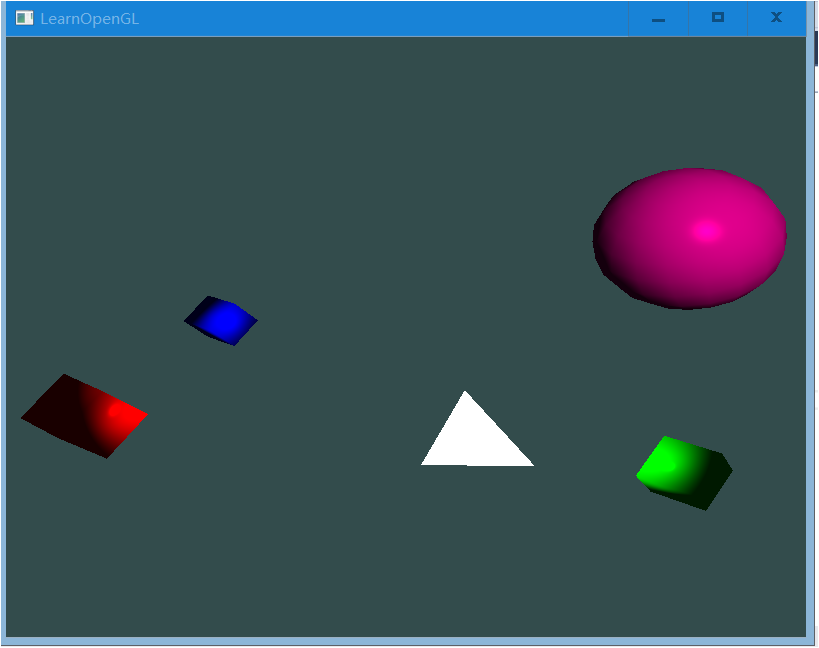
\includegraphics[scale=0.5]{0}
\par z-test enabled, no overlapping\\
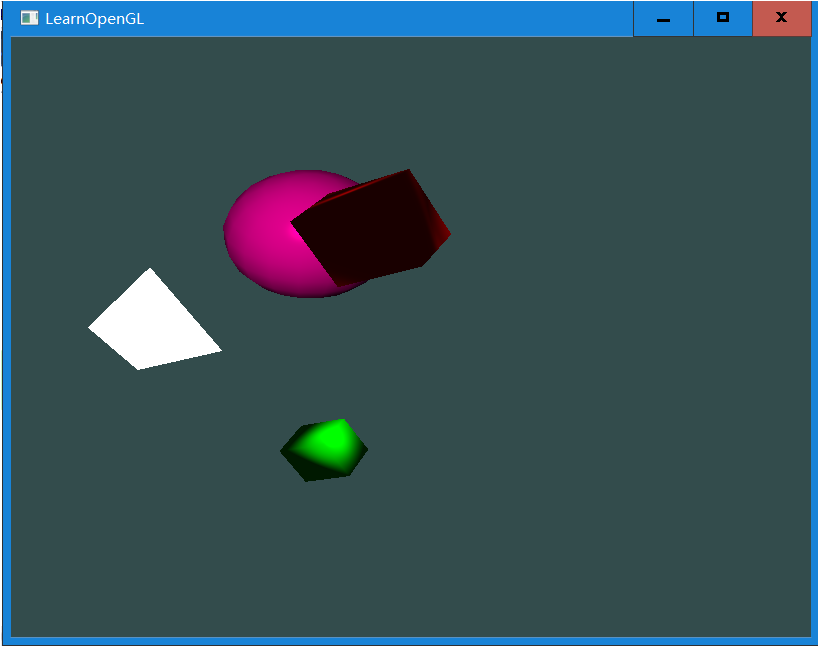
\includegraphics[scale=0.5]{1}
\par Objects rotated. Still get correct shading.\\
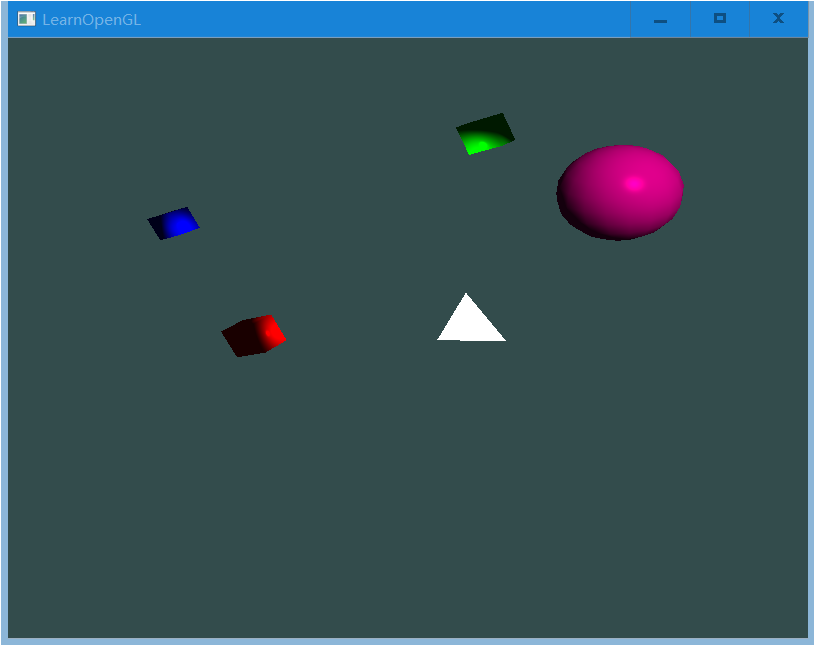
\includegraphics[scale=0.5]{2}
\par Camera moving to back. Still get correct shading.\\
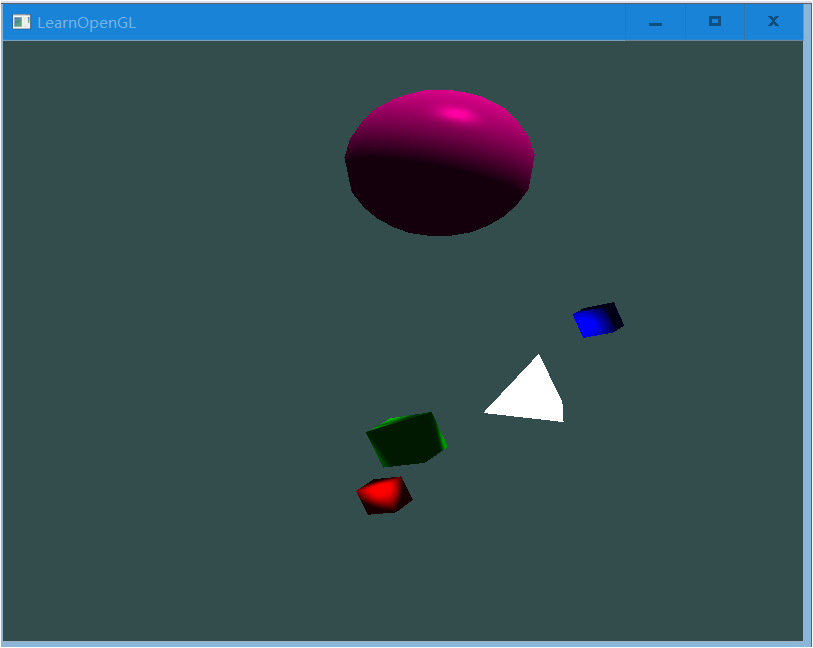
\includegraphics[scale=0.5]{3}

\end{document}
